\section{Introducción}

El Sistema de Protección Social (SPS) busca garantizar un nivel básico en la calidad de vida de los colombianos, a través de la cobertura universal en salud y el aseguramiento de los riesgos de invalidez, vejez y muerte. 

\

La información generada a partir de las cotizaciones es analizada en el contexto económico, social, demográfico, y geográfico de las personas y empresas, y constituye un insumo fundamental para la toma de decisiones de política pública.  Estos resultados identifican los cambios generados del mercado laboral formal a partir de los aportes al SPS y focalizan las personas y empresas más impactadas por los cambios externos o internos a la economía, y con esto optimizar los esfuerzos para la protección y generación del empleo formal en el país. 

\

El documento consta de cinco capítulos que dan respuesta al seguimiento de los aportes: el primero de ellos brinda un panorama general de las dinámicas de los cotizantes, puntualizando en las novedades como pulso de la evolución del mercado laboral formal; el segundo capítulo brinda información de ciclo económico de las empresas y personas dependientes del sector privado e independiente mediante emparejamientos longitudinales de las relaciones laborales con meses previos; el tercer capítulo explora la evolución del aporte al SPS y por ultimo unos anexos técnicos que permiten conocer la evolución de los entornos en otros aspectos sociales, demográficos y económicos del país. 
 
\section{Dinámica general de las cotizaciones}

Esta sección tiene como objetivo resumir el comportamiento general de las cotizaciones para el mes de Diciembre de 2021. Este análisis involucra la descripción del Índice Estacional Medio \footnote{Ver definición en el Anexo \ref{section:anexo:IEM}} como una herramienta desarrollada por la Dirección de Estrategia y Evaluación para el realizar un comparativo mes a mes de la evolución de las cotizaciones dentro de un año típico. La segunda parte se enfoca en identificar los crecimientos en el total de cotizantes diferenciados como independientes y dependientes. La tercera sección describe la evolución que han presentado las novedades discriminadas en sus cinco categorías principales. Este último presenta una evolución de 18 meses para el total de ingresos y retiros, y una descripción de 12 meses para las suspensiones, incapacidades y vacaciones.

%Comportamiento de los cotizantes (tdos los dependientes)
%Comportamiento de algunas novedades  (variaciones anuales y mensuales) 2021, 2020 y 2019. Lo mismo retiros. Bajan los ingresos. Contraste con IEM */

%cuerpo del documento mencionar variaciones anuales. Hablar de variaciones de solo un salario mínimo. 
 %Variaciones mensuales con el total.
%FABIO 
%Tres hojas!  Capitulo 1 
%1 - General con contraste ano tipo
%2- Cotizantes por rango salarial
%3 - Novedaes


\subsection{Índice Estacional Medio (IEM)}

\begin{wrapfigure}{r}{12cm}
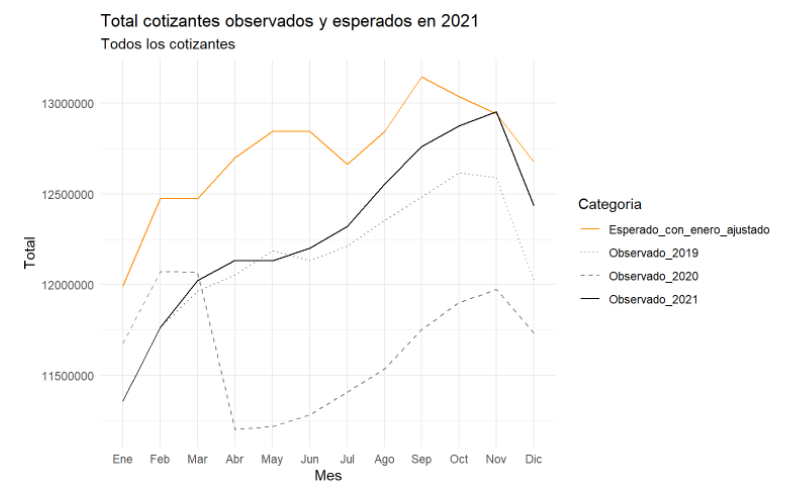
\includegraphics[width = 12.5cm]{figures/01_dinamica/serie_contraste.png}
\caption{Comparativo anual de las cotizaciones}
\label{figura:IEM_Total}
\end{wrapfigure}

El resultado presentado en la figura \ref{figura:IEM_Total} muestra el comportamiento del total de cotizantes para 2019, 2020 y 2021. La evolución 

ANEXO- Dejar los insumos para el IEM (gráfico y tabla con multiplicadores)%

\subsection{Resumen Cotizaciones}

Dejar el resultado general y el contraste con la estimación sin pandemia que usa el IEM, si toca incluir un parrafo general del IEM y de la estimación%

ANEXO- Dejar los insumos para el IEM (gráfico y tabla con multiplicadores)%


\begin{table}[!h]
\centering
\begin{minipage}{0.5\textwidth}
  \centering
  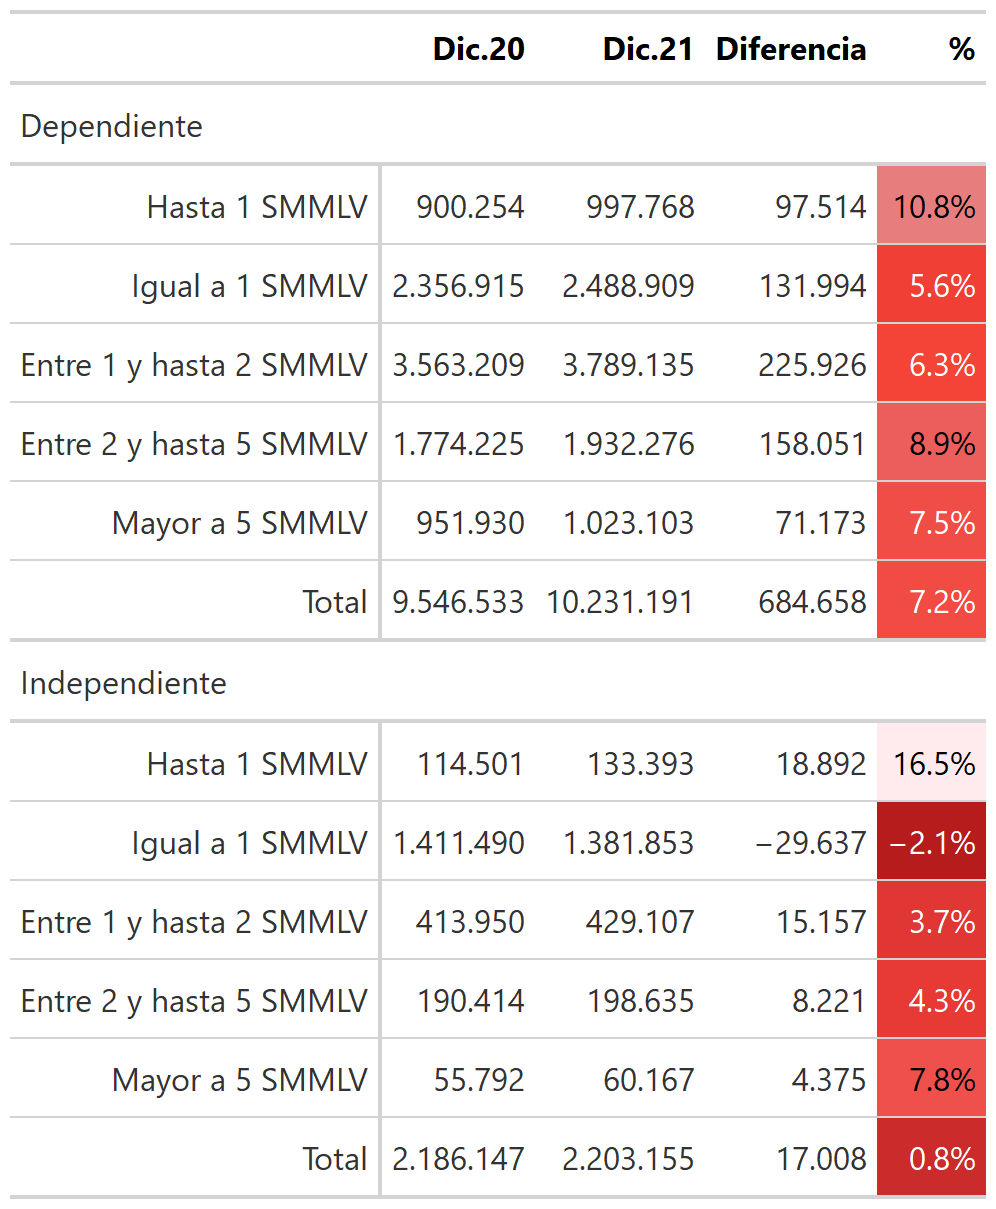
\includegraphics[width=0.6\linewidth]{results/01_dinamica/salida_total_cotizantes.png}
\end{minipage}%
\begin{minipage}{0.5\textwidth}
  \centering
  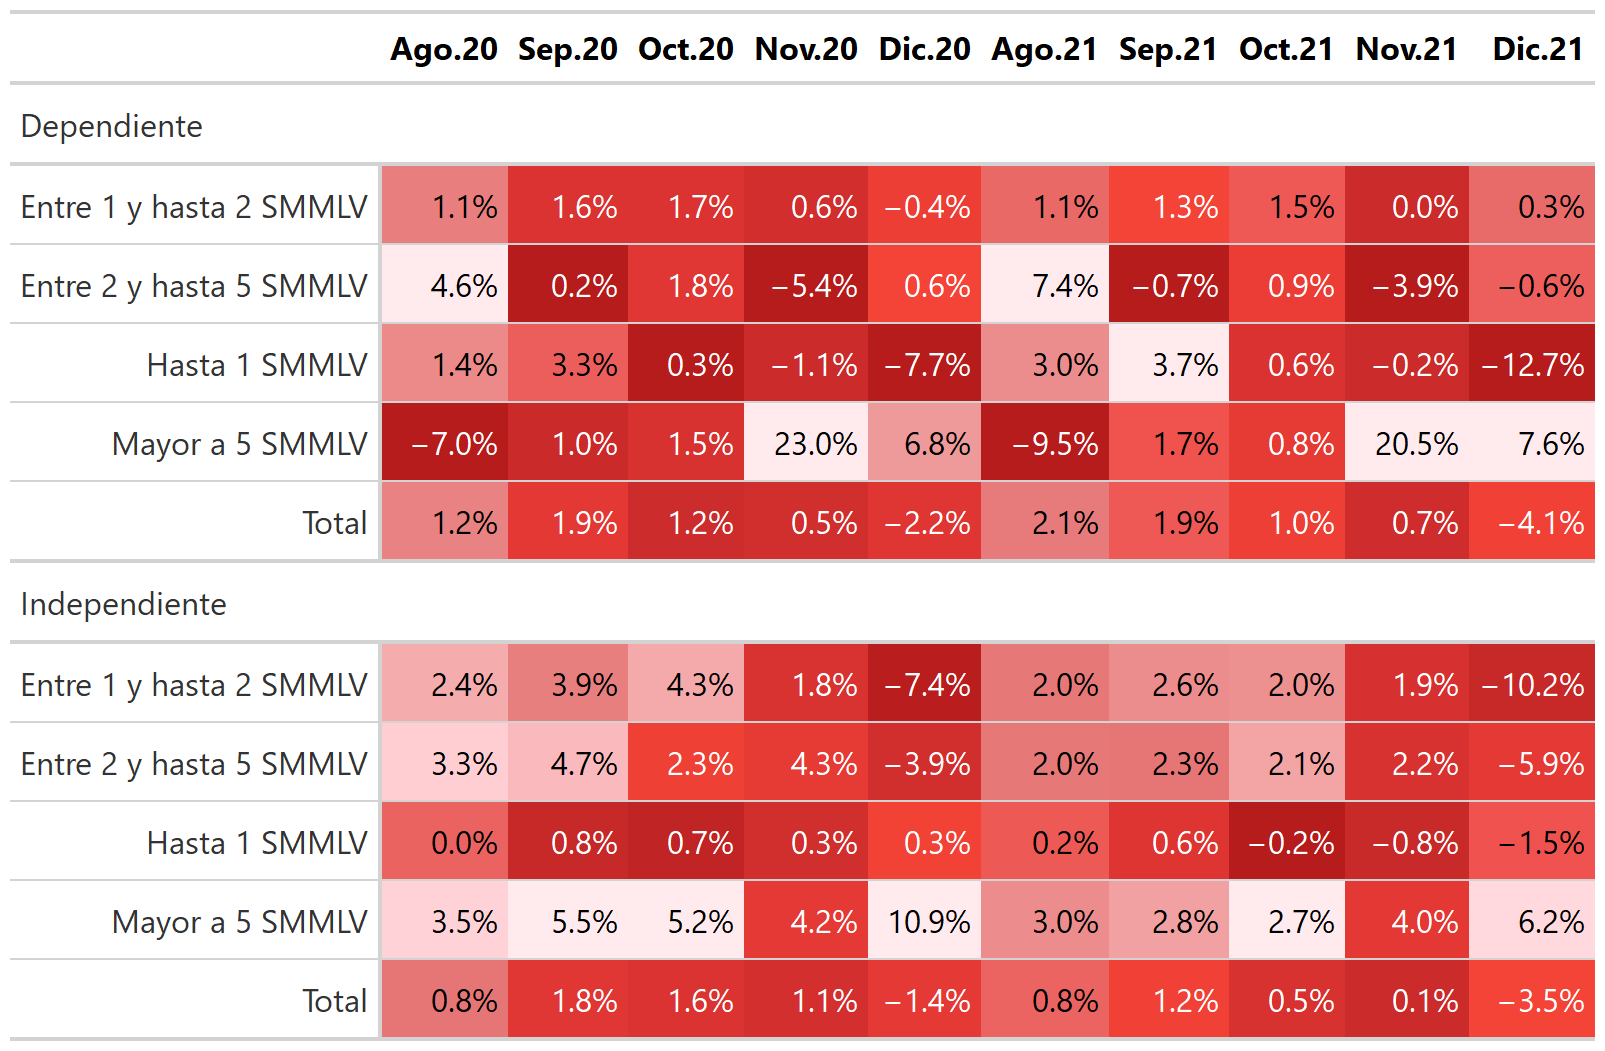
\includegraphics[width=\linewidth]{results/01_dinamica/salida_total_cotizantes_variaciones.png}
\end{minipage}
\caption{Resumen número de cotizantes por rango salarial (IBC). Totales (Izq.), variaciones mensuales (Der.)}
\label{tabla:resumen:cotizantes_rangoIBC}
\end{table}


\subsection{Novedades}

El comportamiento de las novedades en el SPS se analiza a partir de cinco principales características: ingresos, retiros, suspensiones, incapacidades y vacaciones laborales.

\begin{wrapfigure}{r}{0.6\textwidth}
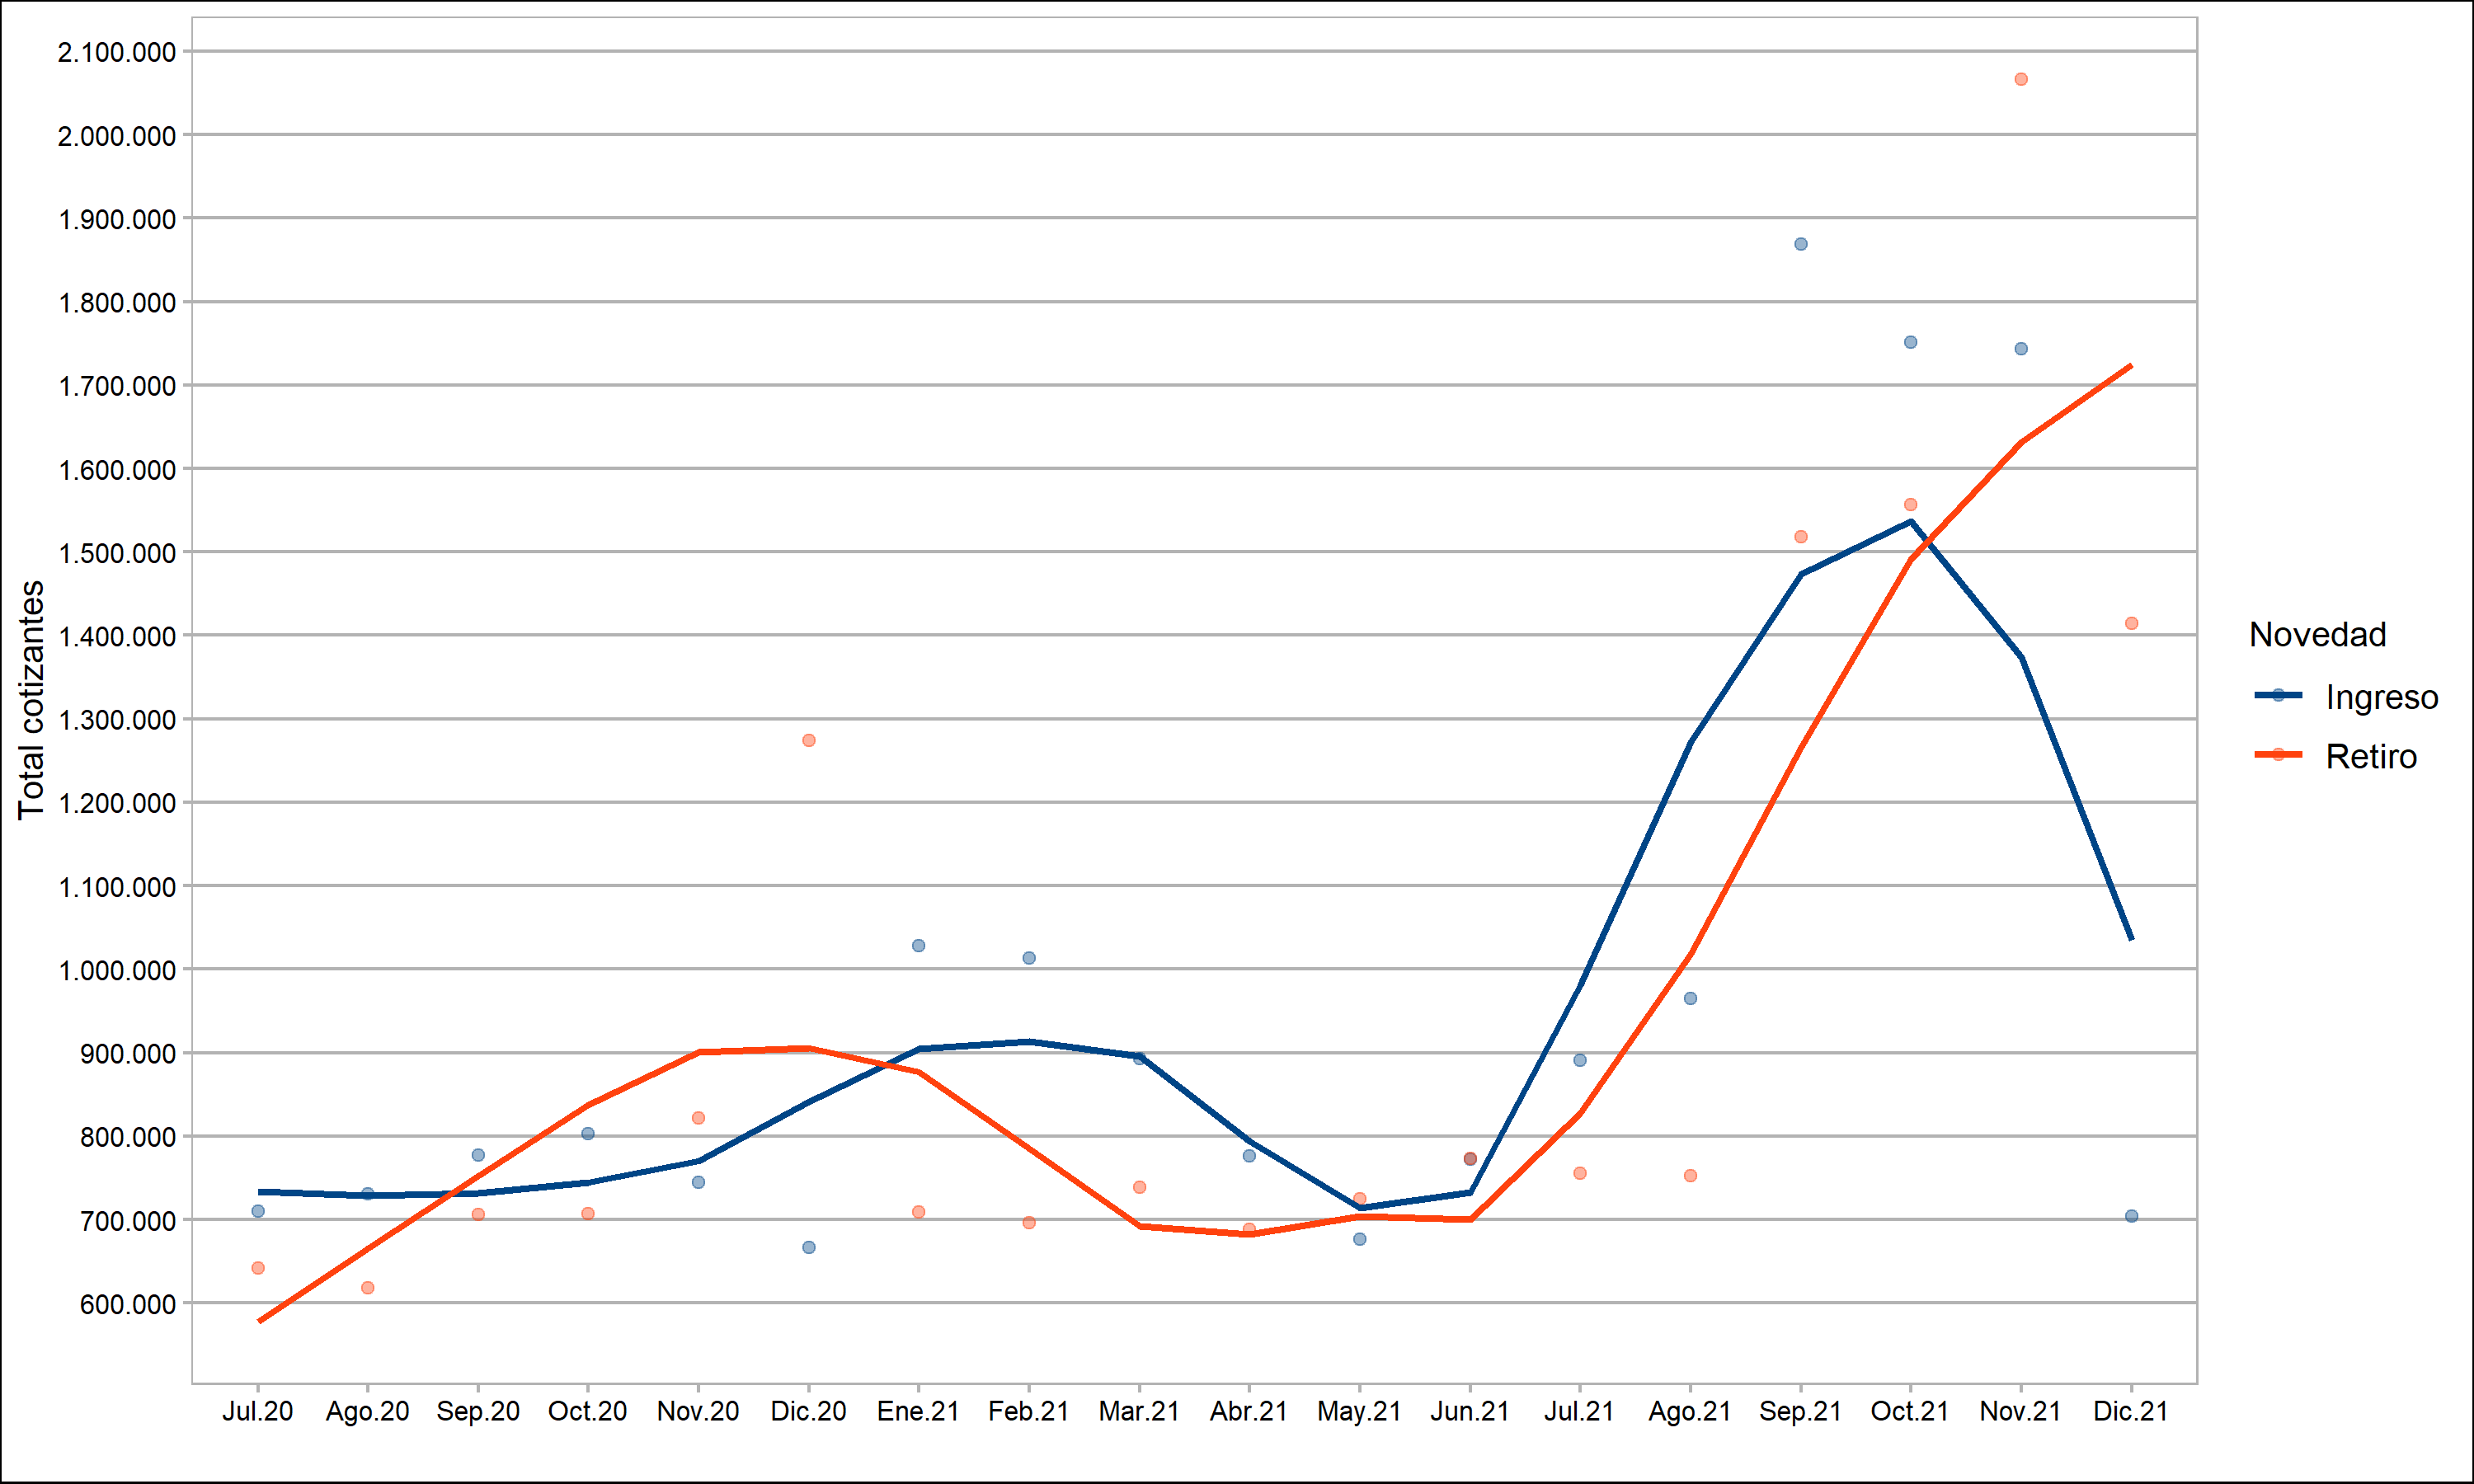
\includegraphics[width = 11.5cm]{figures/01_dinamica/total_novedades_dependientes_ingret.png}
\caption{Comparación del total de novedades para dependientes (ingresos, retiros)}
\label{figura:novedad:sectorprivado:IR}
\end{wrapfigure}
En cuanto a las novedades de los cotizantes independientes se puede observar que desde Junio de 2021 se han incrementado. 

\begin{wrapfigure}{l}{0.6\textwidth}
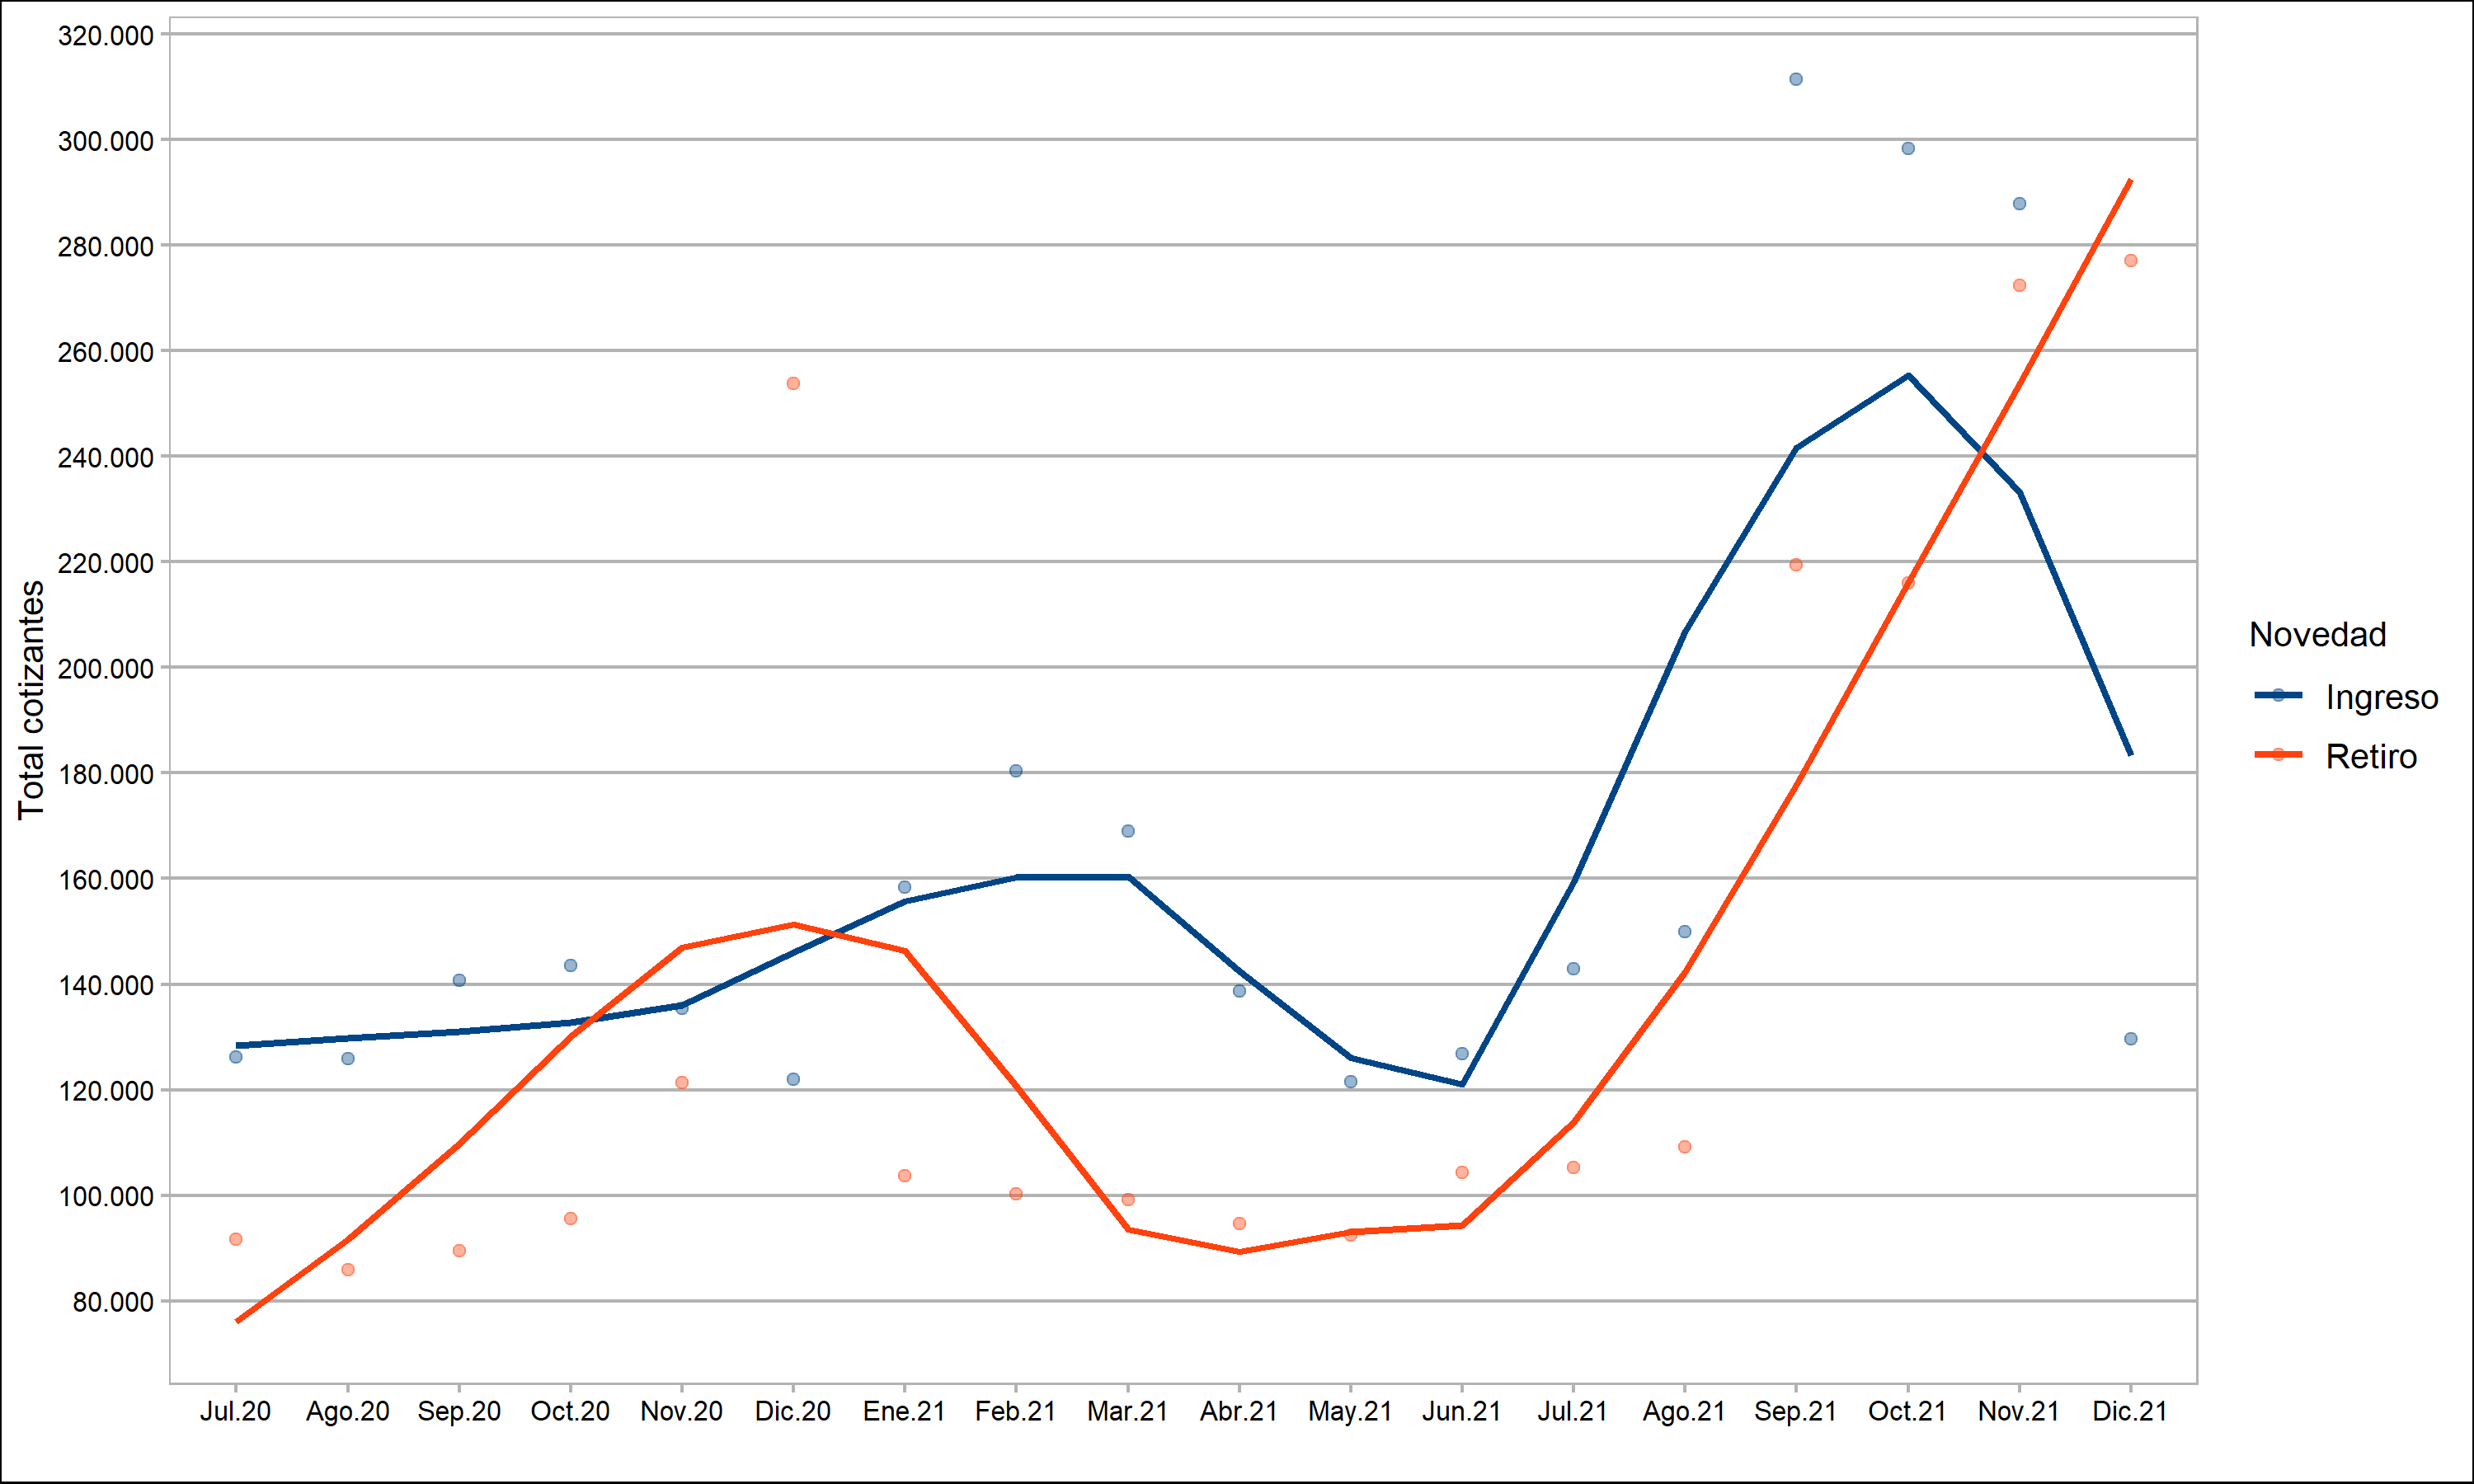
\includegraphics[width = 11.5cm]{figures/01_dinamica/total_novedades_independientes_ingret.png}
\caption{Comparación del total de novedades para independientes}
\label{figura:novedad:sectorprivado:IR}
\end{wrapfigure}


\begin{table}[!h]
\centering
\begin{minipage}{0.5\textwidth}
  \centering
  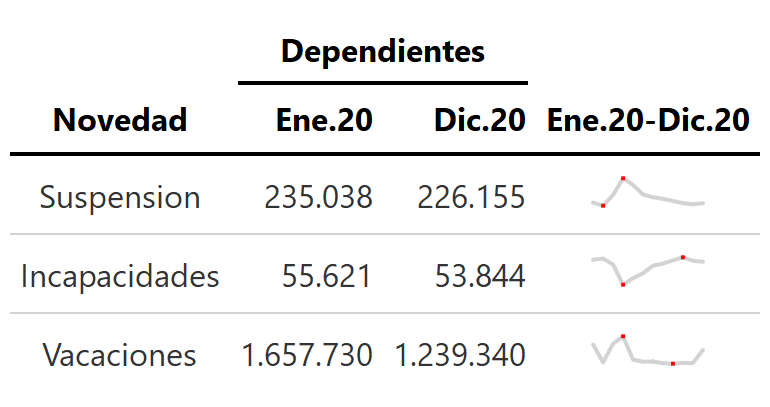
\includegraphics[width=\linewidth]{results/01_dinamica/salida_dependientes_novedades_resto_comparativo.png}
\end{minipage}%
\begin{minipage}{0.5\textwidth}
  \centering
  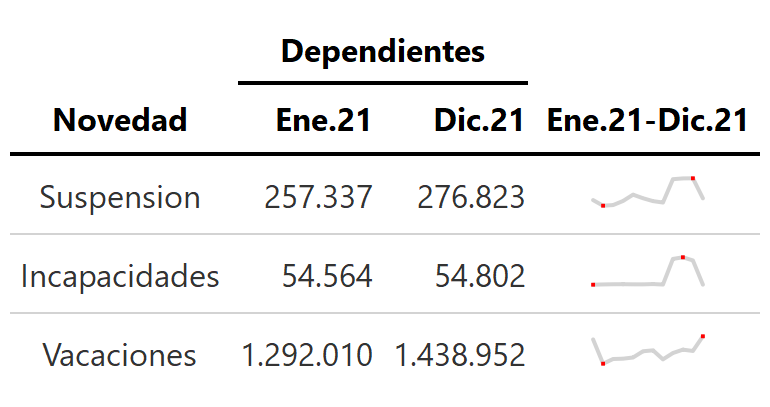
\includegraphics[width=\linewidth]{results/01_dinamica/salida_dependientes_novedades_resto.png}
\end{minipage}
\caption{Total novedades y tendencia anual}
\label{tabla:tabla3}
\end{table}

